
\documentclass{article}
\usepackage[utf8]{inputenc}
\usepackage{mathtext}
\usepackage{amsmath}
\usepackage[colorlinks=true, linkcolor=blue]{hyperref}
\usepackage[T1]{fontenc}
\usepackage[utf8]{inputenc}
\usepackage[english, bulgarian, russian]{babel}
\usepackage{tikz}
\usepackage{pgfplots}
\usepackage{indentfirst}
\usepackage[export]{adjustbox}
\usepackage{lipsum} % sample text
\usepackage{floatflt}
\usepackage{multirow}
\usepackage{geometry} \geometry{verbose,a4paper,tmargin=2cm,bmargin=2cm,lmargin=1.5cm,rmargin=1.5cm}
\setlength{\parindent}{0.65cm}
\setlength{\parskip}{0.15cm}

\usepackage{wrapfig}
\usepackage{array,graphicx,caption}


%Матеша
\usepackage{amsmath,amsfonts,amssymb,amsthm,mathtools} % AMS
\usepackage{icomma} % "Умная" запятая

%\mathtoolsset{showonlyrefs=true} % Показывать номера только у тех формул, на которые есть \eqref{} в тексте.

%% Шрифты
\usepackage{euscript}	 % Шрифт Евклид
\usepackage{mathrsfs} % Красивый матшрифт

%% Свои команды
\DeclareMathOperator{\sgn}{\mathop{sgn}}

%% Перенос знаков в формулах (по Львовскому)
\newcommand*{\hm}[1]{#1\nobreak\discretionary{}
	{\hbox{$\mathsurround=0pt #1$}}{}}


 
\begin{document}
\def\figurename{Рисунок}
\begin{titlepage}
\begin{center}
    {\large МОСКОВСКИЙ ФИЗИКО-ТЕХНИЧЕСКИЙ ИНСТИТУТ (НАЦИОНАЛЬНЫЙ ИССЛЕДОВАТЕЛЬСКИЙ УНИВЕРСИТЕТ)}
\end{center}
\begin{center}
    {\largeФизтех-школа биологической и медицинской физики}
\end{center}

\vspace{1cm}
{\huge
\begin{center}
    {\bf Лабораторная работа по общей физике}\\
    \vspace{0.5cm}
    5.4.2 Исследование энергетического спектра $\beta$-частиц и определение их максимальной энергии при помощи магнитного спектрометра.
\end{center}
}

\vspace{4cm}
\begin{flushright}
{\LARGE Выполнили студенты группы Б06-103:\\ Фитэль Алена \\Флоренская Лидия\\}

\end{flushright}
\vspace{9cm}
\begin{center}
    Долгопрудный, 2023 г.
\end{center}
\end{titlepage}








\newpage
\section{Введение}
\paragraph*{Цель работы:} С помощью магнитного спектрометра исследовать энергетический спектр $\beta$ - частиц при распаде ядер $^{137}$Cs  и определить их максимальную энергию.
\section{Теоретическая справка}


	
	Бета-распадом называется самопроизвольное превращение ядер, при котором их массовое число не изменяется, а заряд увеличивается или уменьшается на единицу. Бета-активные ядра встречаются во всей области значений массового числа $A$, начиная от единицы (свободный нейтрон) и кончая самыми тяжелыми ядрами.	
	
	В данной работе мы будем иметь дело с электронным распадом
	
	\begin{equation*}
		_Z^A\text{X} \; \longrightarrow \;\; _{Z+1}^{\;\;\;\;\,A}\text{X} + e^- + \widetilde{\nu},
	\end{equation*}

	\noindent при котором кроме электрона испускается антинейтрино. Освобождающаяся при $\beta$-распаде энергия делится между электроном, антинейтрино и дочерним ядром, однако доля энергии, передаваемой ядру, исчезающе мала по сравнению с энергией, уносимой электроном и антинейтрино. Практически можно считать, что эти две частицы делят между собой всю освобождающуюся энергию. Поэтому электроны могут иметь любое значение энергии — от нулевой до некоторой максимальной, которая равна энергии, освобождающейся при $\beta$-распаде, являющейся важной физической величиной.
	
	Кинетическая энергия электрона $E$ связана с его импульсом обычным релятивистским соотношением
	\begin{equation}
		E = \sqrt{(pc)^2 + (mc^2)^2} - mc^2.
	\end{equation}

	\begin{wrapfigure}{r}{0.4\textwidth}
		\centering
		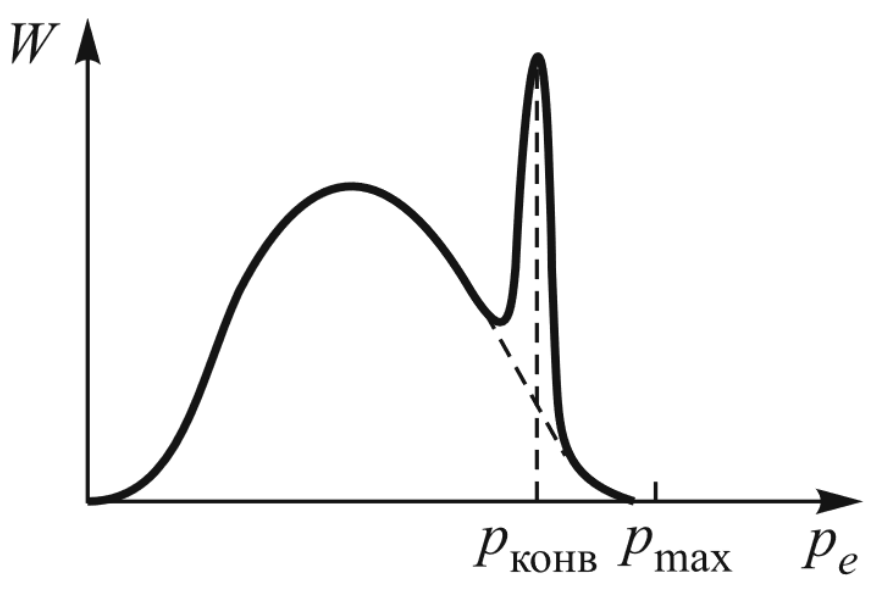
\includegraphics[width=1.2 \linewidth]{pic1.PNG}
		\caption{Форма спектра $\beta$-частиц при разрешенных переходах}
		\label{BetaParticles_Spectre}
	\end{wrapfigure}

	В нерелятивистском приближении формула, выражающая форму $\beta$-спектра приобретает вид:
	\begin{equation}
		\frac{dN}{dE} = \sqrt{E}(E_e - E)^2,
		\label{BetaParticles_dNdE}
	\end{equation}

	\noindent где $E_e$ — максимальная энергия электрона.
	
	Выражение (\ref{BetaParticles_dNdE}) приводит к спектру, имеющему вид широкого колокола (см. рис. \ref{BetaParticles_Spectre}). Кривая плавно отходит от нуля и столь же плавно, по параболе, касается оси абсцисс в области максимальной энергии электронов $E_e$.
	
	
	Дочерние ядра, возникающие в результате $\beta$-распада, нередко оказываются возбужденными. Возбужденные ядра отдают свою энергию либо излучая $\gamma$-квант (энергия которого равна разности энергий начального и конечного уровней), либо передавая избыток энергии одному из электронов с внутренних оболочек атома. Излучаемые в таком процессе электроны имеют строго определенную энергию и называются конверсионными.

	Конверсия чаще всего происходит на оболочках $K$ или $L$. На спектре, представленном на рис. \ref{BetaParticles_Spectre}, видна монохроматическая линия, вызванная электронами конверсии. Ширина этой линии в нашем случае является чисто аппаратурной — по ней можно оценить разрешающую силу спектрометра.
	
	\tocsection{Экспериментальная установка}
	\begin{figure}[h!]
		\centering
		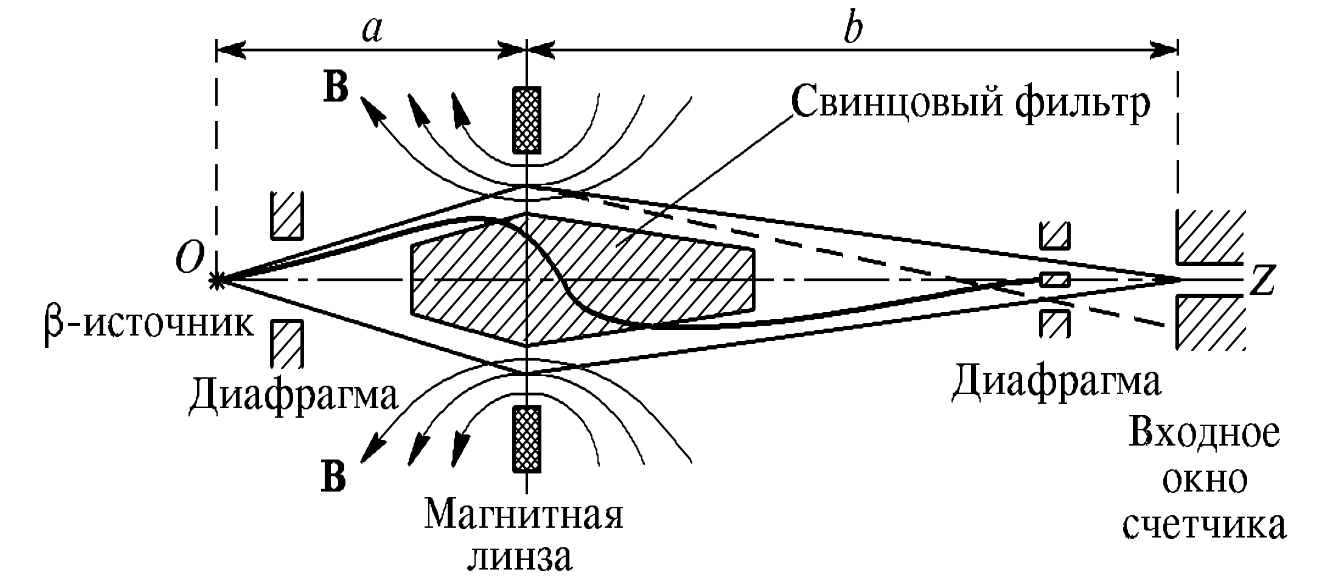
\includegraphics[width=\linewidth]{pic2.PNG}
		\caption{Схема $\beta$-спектрометра с короткой магнитной линзой}
		\label{BetaParticles_Scheme}
	\end{figure}

	Энергию $\beta$-частиц определяют с помощью $\beta$-спектрометров. В работе используется магнитный спектрометр с «короткой линзой». Электроны, испускаемые радиоактивным источником (рис. \ref{BetaParticles_Scheme}), попадают в магнитное поле катушки, ось которой параллельна оси $OZ$ (оси симметрии прибора). Траектории электронов в магнитном поле представляют собой схематически показанные на рисунке сложные спирали, сходящиеся за катушкой в фокусе, расположенном на оси $OZ$. В фокусе установлен детектор электронов. Чувствительным элементом сцинтилляционного счетчика является тонкий кристалл полистирола. При попадании электрона в кристалле возникает световая вспышка -- сцинтилляция, регистрируемая фотоумножителем.
	
	При заданной силе тока на входное окно счетчика фокусируются электроны с определенным импульсом. Электроны, обладающие другими значениями импульса, при этом не сфокусированы и в основном проходят мимо окна (штриховой луч). При изменении тока в катушке на счетчик последовательно фокусируются электроны с разными импульсами. Так как геометрия прибора в течение всего опыта остается неизменной, импульс сфокусированных электронов пропорционален величине тока $I$:
	\begin{equation}
		p_e = kI.
		\label{BetaParticles_pkI}
	\end{equation}
Из-за конечных размеров источника, диафрагм и окна счетчика, а также вследствие аберраций при заданной величине фокусного расстояния на счетчик попадают электроны с импульсами, лежащими внутри некоторого интервала от $p_e - \Delta p_e/2$ до $p_e + \Delta p_e/2$. Величина $\Delta p_e$ -- ширина интервала импульсов, регистрируемых при заданном значении тока, -- называется разрешающей способностью $\beta$-спектрометра.
	
	Ширина интервала $\Delta p_e$, регистрируемого спектрометром, пропорциональна величине импульса.
	
	В результате попадания электронов в сцинтиллятор на выходе фотоумножителя появляются электрические импульсы, которые заносятся в память персонального компьютера и выводятся на экран монитора. Давление в спектрометре поддерживается на уровне около 0,1 Тор и измеряется термопарным вакуумметром. Лучший вакуум в приборе не нужен, поскольку уже при этом давлении потери энергии электронов малы и их рассеяние незначительно. Откачка осуществляется форвакуумным насосом. Магнитная линза питается постоянным током от выпрямителя. Высокое напряжение на ФЭУ или газоразрядный счетчик подается от стабилизированного выпрямителя.
	



\section{Ход работы}
	\begin{enumerate}
		\item Откачаем воздух из полости спектрометра. Включим формирователь импульсов, питание магнитной линзы.	
		\item Приступим к подробному измерению $\beta$-спектра. Результаты приведены в Таблице \ref{BetaParticles_ExpTable} (Приложение) и проиллюстрированы на Рисунке \ref{fig:no_int} . 


\begin{figure}[h!]
\begin{center}
\begin{minipage}[h!]{0.45\linewidth}
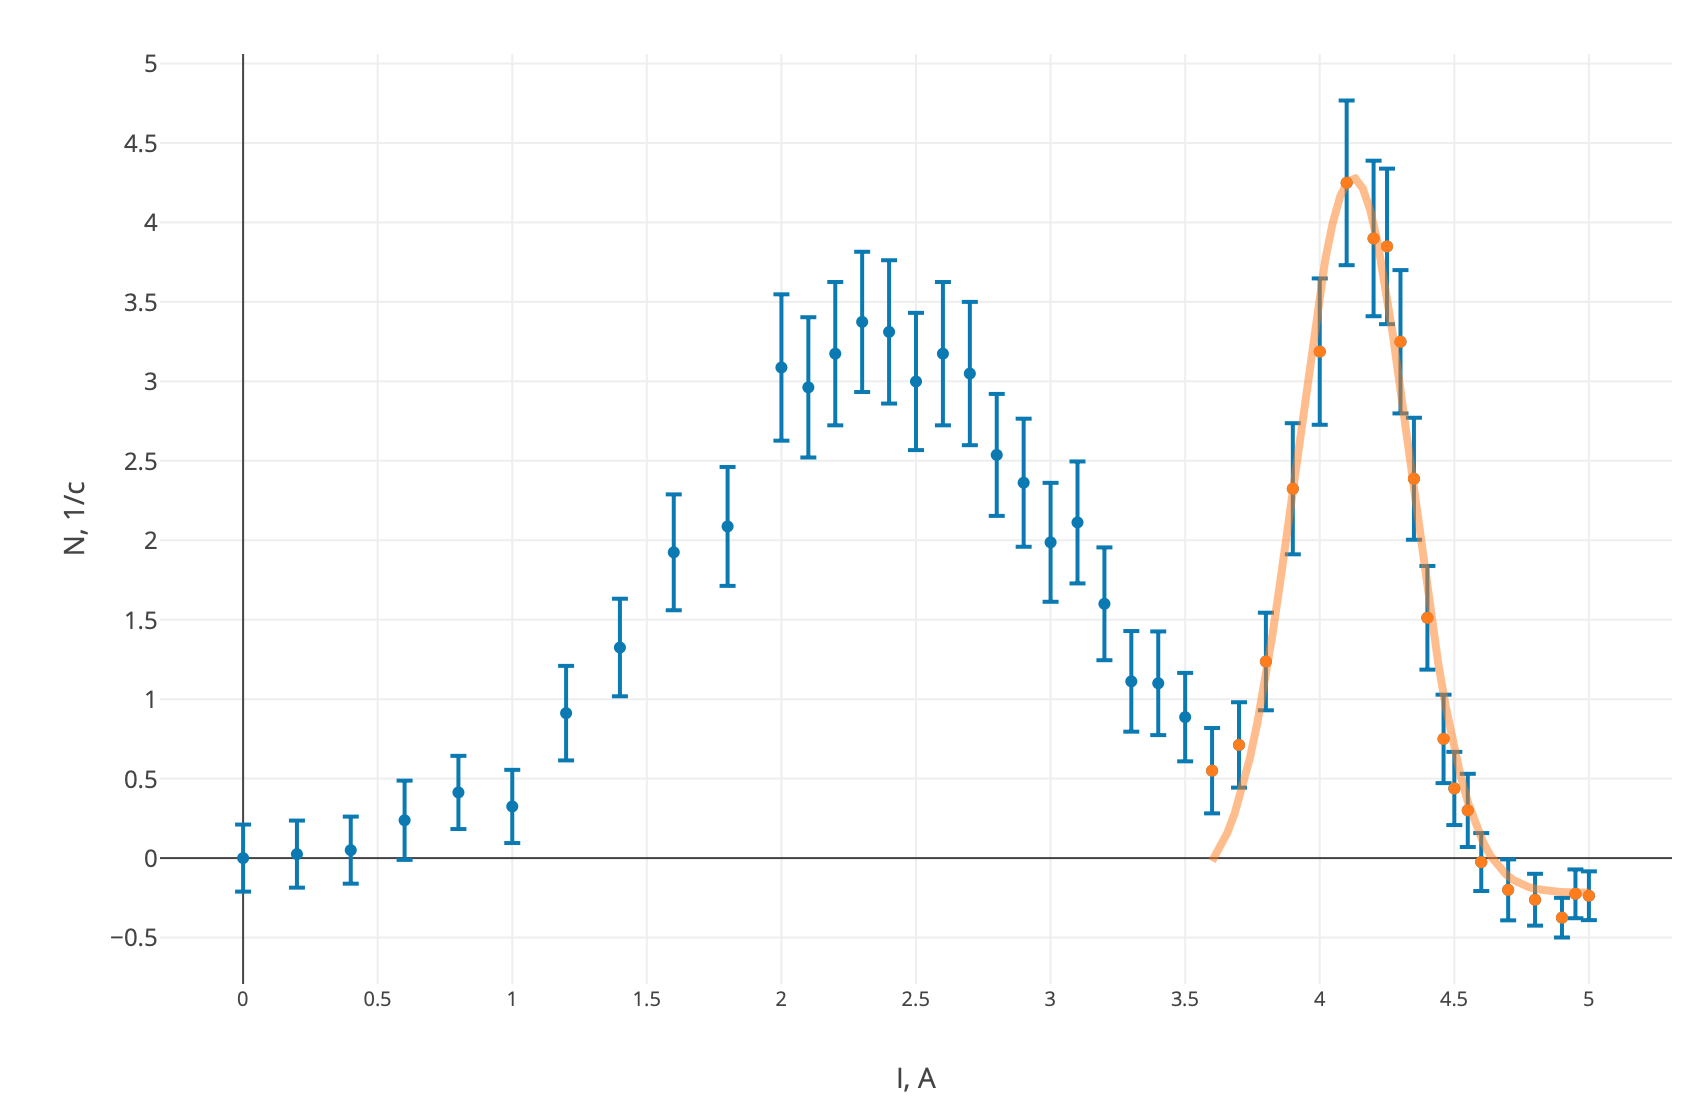
\includegraphics[scale = 0.37]{N_I.png}
\caption{$\beta$-спектр (с вычетом фона)}
\label{fig:no_int}
\end{minipage}
\hfill
\begin{minipage}[h]{0.45\linewidth}
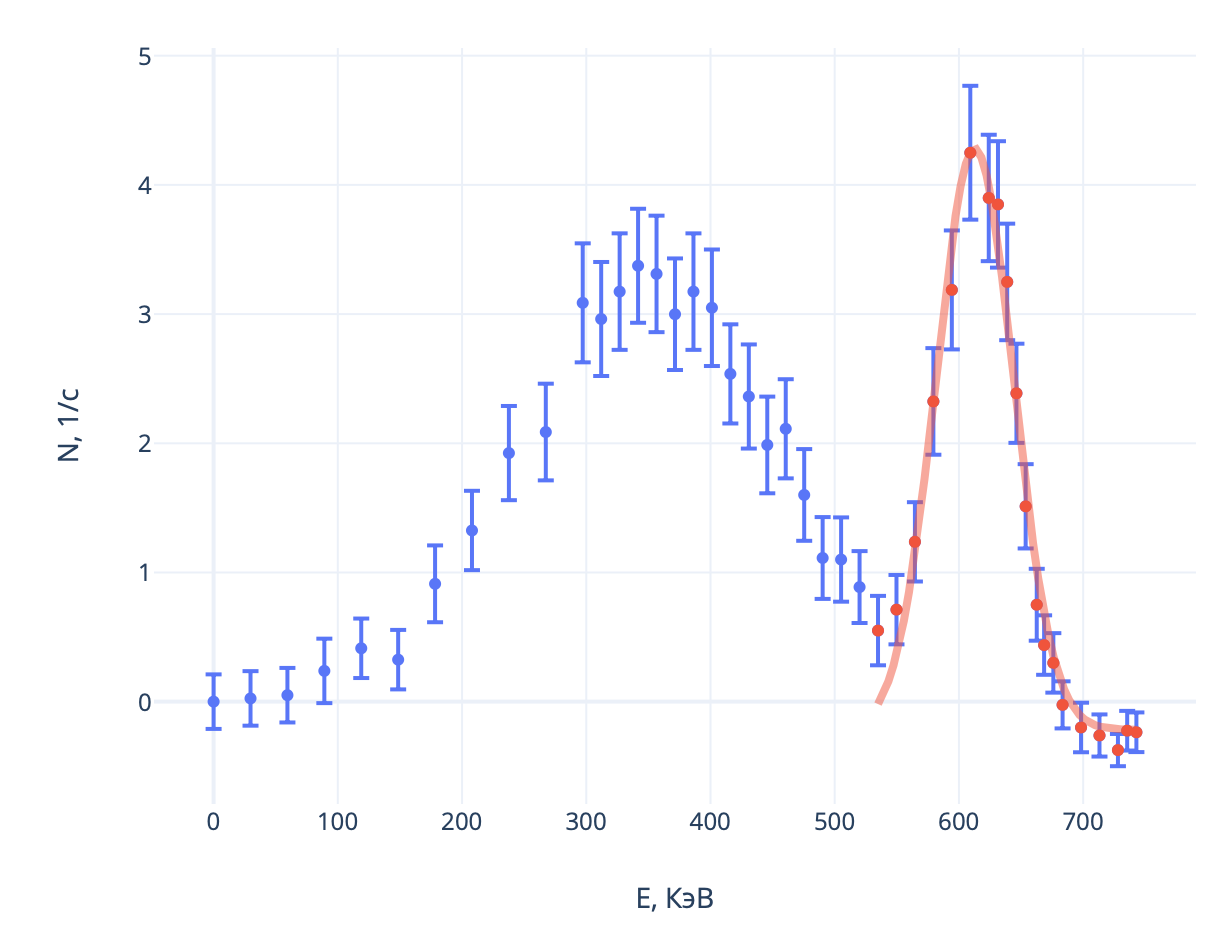
\includegraphics[scale = 0.4]{N_E.png}
			\caption{График зависимости числа $N$ частиц от их энергии $E$}
\label{fig:no_int1}
\end{minipage}
\end{center}
\end{figure}







	
		\item  Коэффициент $k$ ($kc$) из зависимости (3)  определим по известной (табличное значение) конверсионной линии:
			$$624 \ \text{кэВ} = kcI_0,$$
		где $c$ -- скорость света, $I_0 = 4,20 \pm 0,02$ А -- сила тока, при которой наблюдается конверсионный пик:
		\begin{equation*}
			kc = 149 \pm 7 \frac{\text{кэВ}}{\text{A}},
		\end{equation*}
	 	
	 	\item Теперь, зная эту каллибровочную константу, построим график Ферми-Кюри (Рисунок \ref{fig:no_int2}, Таблица \ref{tab:my-table} (Приложение)) с помощью взвешенного МНК, то есть зависимость величины $\frac{\sqrt{N}}{p^{3/2}}$ от энергии электрона $E$. Из него, по пересечению с осью абсцисс, можно определить максимальную энергию $\beta$-частиц. Анализ спектра в координатах $ N(T)$ (Рисунок \ref{fig:no_int1}) в нашем случае даст грубый результат для оценки максимальной энергии, так как придётся ограничиться исследованием точек у самой верхней границы спектра. График Ферми-Кюри позволяет избежать столь грубых оценок и учесть больше точек, поэтому для подсчета максимума энергии мы будем использовать именно его.
		
	


		\begin{figure}[h!]
			\centering
			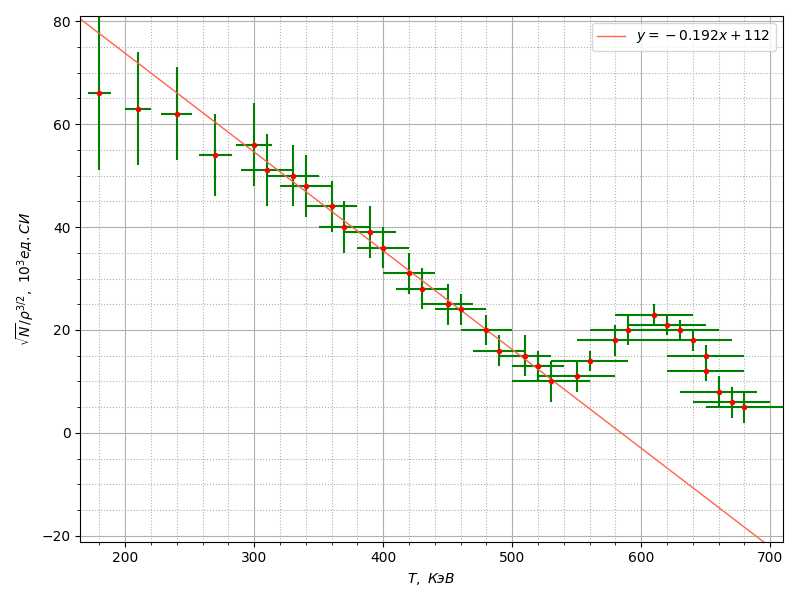
\includegraphics[scale = 0.67]{5.4.2 (2).png}
			\caption{График Ферми-Кюри}
            \label{fig:no_int2}
		\end{figure}
	
		Получаем следующие коэффициенты из аппроксимации прямой графика Ферми-Кюри $y = Ax + B$:
		\begin{itemize}
			\item $A = (-0,192 \pm 0,005)$ $(\frac{\text{м}}{\text{с} \cdot \text{эВ}^2})^{3/2 }$
			
			\item $B = (112 \pm 2) (\frac{\text{м}}{\text{с} \cdot \text{эВ}})^{3/2 }$
		
            \end{itemize}
  Максимальная энергия $\beta$-частиц определяется пересечением прямой с осью абсцисс:
		\begin{equation*}
			E_\text{max} = -\frac{B}{A}
		\end{equation*}
		\begin{equation*}
			\boxed{E_\text{max} = (584 \pm 18) \text{ кэВ}}
		\end{equation*}
		
		
		Табличное значение: $E_\text{max}^\text{истин} = 634 \text{ кэВ}$.
	\end{enumerate}
	
	
	\section{Вывод}
 \begin{itemize}
     \item В результате выполнения лабораторной работы был изучен энергетический спектр $\beta$ - частиц при распаде ядер $^{137}$Cs.  
	
\itemМы экспериментально удостоверились в том,  что спектр $\beta$ - частиц имеет вид широкого купола,  причем данная кривая плавно касается оси абсцисс в области максимальной энергии электронов $E_e$. Также в спектре отчетливо наблюдается конверсионный пик.


\item Была определена максимальная энергия $\beta$-частиц при данном распаде: $E_\text{max} = (584 \pm 18)$ кэВ. Относительная погрешность составляет $ 9\%$ (табличное значение величиныэ: $E_\text{max}^\text{истин} = 634 \text{ кэВ}$ ).


 \end{itemize}
	 

\newpage
\section{Приложение}
\begin{table}[h!]
\centering
\begin{tabular}{|c|r|c|r|r|r|r|}
\hline
№ &
  \multicolumn{1}{c|}{$ I, $ А} &
  $ \sigma_l $, А &
 \multicolumn{1}{c|}{$ N $, 1/c} &
  \multicolumn{1}{l|}{$ \sigma_N $, 1/c} &
  \multicolumn{1}{c|}{$ N - N_f$, 1/c} &
  \multicolumn{1}{c|}{$ \sigma_{N-N_f}$, 1/c} \\ \hline
1                        & 0    & 0.02 & 0.7  & 0.2  & 0    & 0.3 \\ \hline
2                        & 0.2  & 0.02 & 0.8  & 0.2  & 0    & 0.3 \\ \hline
3                        & 0.4  & 0.02 & 0.8  & 0.2  & 0.1  & 0.3 \\ \hline
4                        & 0.6  & 0.02 & 1    & 0.2  & 0.2  & 0.4 \\ \hline
5                        & 0.8  & 0.02 & 1.2  & 0.2  & 0.4  & 0.3 \\ \hline
6                        & 1    & 0.02 & 1.1  & 0.2  & 0.3  & 0.3 \\ \hline
7                        & 1.2  & 0.02 & 1.6  & 0.3  & 0.9  & 0.4 \\ \hline
8                        & 1.4  & 0.02 & 2.1  & 0.3  & 1.3  & 0.4 \\ \hline
9                        & 1.6  & 0.02 & 2.7  & 0.4  & 1.9  & 0.5 \\ \hline
10                       & 1.8  & 0.02 & 2.8  & 0.4  & 2.1  & 0.5 \\ \hline
11                       & 2    & 0.02 & 3.8  & 0.5  & 3.1  & 0.7 \\ \hline
12                       & 2.1  & 0.02 & 3.7  & 0.4  & 3    & 0.6 \\ \hline
13                       & 2.2  & 0.02 & 3.9  & 0.5  & 3.2  & 0.6 \\ \hline
14                       & 2.3  & 0.02 & 4.1  & 0.4  & 3.4  & 0.6 \\ \hline
15                       & 2.4  & 0.02 & 4    & 0.5  & 3.3  & 0.6 \\ \hline
16                       & 2.5  & 0.02 & 3.7  & 0.4  & 3    & 0.6 \\ \hline
17                       & 2.6  & 0.02 & 3.9  & 0.5  & 3.2  & 0.6 \\ \hline
18                       & 2.7  & 0.02 & 3.8  & 0.5  & 3    & 0.6 \\ \hline
19                       & 2.8  & 0.02 & 3.3  & 0.4  & 2.5  & 0.5 \\ \hline
20                       & 2.9  & 0.02 & 3.1  & 0.4  & 2.4  & 0.6 \\ \hline
21                       & 3    & 0.02 & 2.7  & 0.4  & 2    & 0.5 \\ \hline
22                       & 3.1  & 0.02 & 2.8  & 0.4  & 2.1  & 0.5 \\ \hline
23                       & 3.2  & 0.02 & 2.3  & 0.4  & 1.6  & 0.5 \\ \hline
24                       & 3.3  & 0.02 & 1.8  & 0.3  & 1.1  & 0.4 \\ \hline
25                       & 3.4  & 0.02 & 1.8  & 0.3  & 1.1  & 0.5 \\ \hline
26                       & 3.5  & 0.02 & 1.6  & 0.3  & 0.9  & 0.4 \\ \hline
27                       & 3.6  & 0.02 & 1.3  & 0.3  & 0.6  & 0.4 \\ \hline
28                       & 3.7  & 0.02 & 1.4  & 0.3  & 0.7  & 0.4 \\ \hline
29                       & 3.8  & 0.02 & 2    & 0.3  & 1.2  & 0.4 \\ \hline
30                       & 3.9  & 0.02 & 3.1  & 0.4  & 2.3  & 0.6 \\ \hline
31                       & 4    & 0.02 & 3.9  & 0.5  & 3.2  & 0.7 \\ \hline
32                       & 4.1  & 0.02 & 5    & 0.5  & 4.2  & 0.7 \\ \hline
33                       & 4.2  & 0.02 & 4.6  & 0.5  & 3.9  & 0.7 \\ \hline
\multicolumn{1}{|r|}{34} & 4.25 & 0.02 & 4.6  & 0.5  & 3.8  & 0.7 \\ \hline
\multicolumn{1}{|r|}{35} & 4.3  & 0.02 & 4    & 0.5  & 3.2  & 0.7 \\ \hline
\multicolumn{1}{|r|}{36} & 4.35 & 0.02 & 3.1  & 0.5  & 2.4  & 0.6 \\ \hline
\multicolumn{1}{|r|}{37} & 4.4  & 0.02 & 2.2  & 0.4  & 1.5  & 0.5 \\ \hline
\multicolumn{1}{|r|}{38} & 4.46 & 0.02 & 1.5  & 0.3  & 0.8  & 0.5 \\ \hline
\multicolumn{1}{|r|}{39} & 4.5  & 0.02 & 1.2  & 0.3  & 0.4  & 0.4 \\ \hline
\multicolumn{1}{|r|}{40} & 4.55 & 0.02 & 1    & 0.2  & 0.3  & 0.3 \\ \hline
\multicolumn{1}{|r|}{41} & 4.6  & 0.02 & 0.71 & 0.18 & 0    & 0.3 \\ \hline
\multicolumn{1}{|r|}{42} & 4.7  & 0.02 & 0.54 & 0.19 & -0.2 & 0.3 \\ \hline
\multicolumn{1}{|r|}{43} & 4.8  & 0.02 & 0.48 & 0.16 & -0.3 & 0.2 \\ \hline
\multicolumn{1}{|r|}{44} & 4.9  & 0.02 & 0.36 & 0.12 & -0.4 & 0.2 \\ \hline
\multicolumn{1}{|r|}{45} & 4.95 & 0.02 & 0.51 & 0.15 & -0.2 & 0.2 \\ \hline
\multicolumn{1}{|r|}{46} & 5    & 0.02 & 0.5  & 0.15 & -0.2 & 0.2 \\ \hline
\end{tabular}
\caption{Результаты измерений.}
\label{BetaParticles_ExpTable}
\end{table}


  \begin{table}[h!]
\centering
\begin{tabular}{|c|r|r|r|r|r|r|r|}
\hline
№ &
  \multicolumn{1}{c|}{$ I, $ А} &
  \multicolumn{1}{c|}{$ pc,$ кэВ} &
  \multicolumn{1}{c|}{$ \sigma_{pc}$, кэВ} &
  \multicolumn{1}{c|}{$ T $, кэВ} &
  \multicolumn{1}{c|}{$ \sigma_T $, кэВ} &
  \multicolumn{1}{c|}{$ f$, $(\frac{\text{м}}{\text{с} \cdot \text{эВ}})^{3/2 }$} &
  \multicolumn{1}{c|}{$ \sigma_f$, $(\frac{\text{м}}{\text{с} \cdot \text{эВ}})^{3/2 }$}\\ \hline
1 &
  0 &
  \multicolumn{1}{l|}{-} &
  \multicolumn{1}{l|}{-} &
  \multicolumn{1}{l|}{-} &
  \multicolumn{1}{l|}{-} &
  \multicolumn{1}{l|}{-} &
  \multicolumn{1}{l|}{-} \\ \hline
2                        & 0.2  & 30  & 3  & 30  & 3  & 160                    & 963                    \\ \hline
3                        & 0.4  & 60  & 4  & 60  & 4  & 80                     & 240                    \\ \hline
4                        & 0.6  & 90  & 5  & 90  & 5  & 100                    & 80                     \\ \hline
5                        & 0.8  & 120 & 6  & 120 & 6  & 81                     & 30                     \\ \hline
6                        & 1    & 150 & 8  & 150 & 8  & 52                     & 24                     \\ \hline
7                        & 1.2  & 180 & 9  & 180 & 9  & 66                     & 15                     \\ \hline
8                        & 1.4  & 210 & 10 & 210 & 10 & 63                     & 11                     \\ \hline
9                        & 1.6  & 240 & 12 & 240 & 12 & 62                     & 9                      \\ \hline
10                       & 1.8  & 270 & 13 & 270 & 13 & 54                     & 8                      \\ \hline
11                       & 2    & 300 & 14 & 300 & 14 & 56                     & 8                      \\ \hline
12                       & 2.1  & 310 & 20 & 310 & 20 & 51                     & 7                      \\ \hline
13                       & 2.2  & 330 & 20 & 330 & 20 & 50                     & 6                      \\ \hline
14                       & 2.3  & 340 & 20 & 340 & 20 & 48                     & 6                      \\ \hline
15                       & 2.4  & 360 & 20 & 360 & 20 & 44                     & 5                      \\ \hline
16                       & 2.5  & 370 & 20 & 370 & 20 & 40                     & 5                      \\ \hline
17                       & 2.6  & 390 & 20 & 390 & 20 & 39                     & 5                      \\ \hline
18                       & 2.7  & 400 & 20 & 400 & 20 & 36                     & 4                      \\ \hline
19                       & 2.8  & 420 & 20 & 420 & 20 & 31                     & 4                      \\ \hline
20                       & 2.9  & 430 & 20 & 430 & 20 & 28                     & 4                      \\ \hline
21                       & 3    & 450 & 20 & 450 & 20 & 25                     & 4                      \\ \hline
22                       & 3.1  & 460 & 20 & 460 & 20 & 24                     & 3                      \\ \hline
23                       & 3.2  & 480 & 20 & 480 & 20 & 20                     & 3                      \\ \hline
24                       & 3.3  & 490 & 20 & 490 & 20 & 16                     & 3                      \\ \hline
25                       & 3.4  & 510 & 20 & 510 & 20 & 15                     & 4                      \\ \hline
26                       & 3.5  & 520 & 20 & 520 & 20 & 13                     & 3                      \\ \hline
27                       & 3.6  & 530 & 30 & 530 & 30 & 10                     & 4                      \\ \hline
28                       & 3.7  & 550 & 30 & 550 & 30 & 11                     & 3                      \\ \hline
29                       & 3.8  & 560 & 30 & 560 & 30 & 14                     & 2                      \\ \hline
30                       & 3.9  & 580 & 30 & 580 & 30 & 18                     & 3                      \\ \hline
31                       & 4    & 590 & 30 & 590 & 30 & 20                     & 3                      \\ \hline
32                       & 4.1  & 610 & 30 & 610 & 30 & 23                     & 2                      \\ \hline
33                       & 4.2  & 620 & 30 & 620 & 30 & 21                     & 2                      \\ \hline
\multicolumn{1}{|r|}{34} & 4.25 & 630 & 30 & 630 & 30 & 20                     & 2                      \\ \hline
\multicolumn{1}{|r|}{35} & 4.3  & 640 & 30 & 640 & 30 & 18                     & 2                      \\ \hline
\multicolumn{1}{|r|}{36} & 4.35 & 650 & 30 & 650 & 30 & 15                     & 2                      \\ \hline
\multicolumn{1}{|r|}{37} & 4.4  & 650 & 30 & 650 & 30 & 12                     & 2                      \\ \hline
\multicolumn{1}{|r|}{38} & 4.46 & 660 & 30 & 660 & 30 & 8                      & 3                      \\ \hline
\multicolumn{1}{|r|}{39} & 4.5  & 670 & 30 & 670 & 30 & 6                      & 3                      \\ \hline
\multicolumn{1}{|r|}{40} & 4.55 & 680 & 30 & 680 & 30 & 5                      & 3                      \\ \hline
\multicolumn{1}{|r|}{41} & 4.6  & 680 & 30 & 680 & 30 & \multicolumn{1}{l|}{-} & \multicolumn{1}{l|}{-} \\ \hline
\multicolumn{1}{|r|}{42} & 4.7  & 700 & 30 & 700 & 30 & \multicolumn{1}{l|}{-} & \multicolumn{1}{l|}{-} \\ \hline
\multicolumn{1}{|r|}{43} & 4.8  & 710 & 30 & 710 & 30 & \multicolumn{1}{l|}{-} & \multicolumn{1}{l|}{-} \\ \hline
\multicolumn{1}{|r|}{44} & 4.9  & 730 & 30 & 730 & 30 & \multicolumn{1}{l|}{-} & \multicolumn{1}{l|}{-} \\ \hline
\multicolumn{1}{|r|}{45} & 4.95 & 740 & 40 & 740 & 40 & \multicolumn{1}{l|}{-} & \multicolumn{1}{l|}{-} \\ \hline
\multicolumn{1}{|r|}{46} & 5    & 740 & 40 & 740 & 40 & \multicolumn{1}{l|}{-} & \multicolumn{1}{l|}{-} \\ \hline
\end{tabular}
\caption{Вычисление энергии и импульса для соответствующего измерения, данные для построения графика Ферми-Кюри. }
\label{tab:my-table}
\end{table}



\end{document}
